\section{Benchmarking}\label{sec:benchmarking}

We tested performance of mentioned acceleration methods in different environments. Implementation status and reason if not implemented is shown in table~\ref{tab:implemented}. Tested JS environments and their versions are described in table~\ref{tab:versions}.

\begin{wraptable}{r}{7.5cm}
    \vspace{-0.5cm}
    \begin{threeparttable}
        \caption{Analyzed acceleration methods and environments.}
        \label{tab:implemented}
        \setlength{\tabcolsep}{0.3em}
        \begin{tabularx}{7.5cm}{lllll }%
            \hline
                         & Chrome                            & Firefox                           & Node                              & Deno                              \\
            \hline
            Sequential   & \textcolor{blue}{\cmark}          & \textcolor{blue}{\cmark}          & \textcolor{blue}{\cmark}          & \textcolor{blue}{\cmark}          \\
            Native addon & \textcolor{red}{\xmark} \tnote{1} & \textcolor{red}{\xmark} \tnote{1} & \textcolor{blue}{\cmark}          & \textcolor{red}{\xmark} \tnote{2} \\
            asm.js       & \textcolor{blue}{\cmark}          & \textcolor{blue}{\cmark}          & \textcolor{blue}{\cmark}          & \textcolor{red}{\xmark} \tnote{2} \\
            WASM         & \textcolor{blue}{\cmark}          & \textcolor{blue}{\cmark}          & \textcolor{blue}{\cmark}          & \textcolor{red}{\xmark} \tnote{2} \\
            WASM+SIMD    & \textcolor{blue}{\cmark}          & \textcolor{blue}{\cmark}          & \textcolor{blue}{\cmark}          & \textcolor{red}{\xmark} \tnote{2} \\
            Workers      & \textcolor{blue}{\cmark}          & \textcolor{blue}{\cmark}          & \textcolor{blue}{\cmark}          & \textcolor{blue}{\cmark}          \\
            WebGL        & \textcolor{blue}{\cmark}          & \textcolor{blue}{\cmark}          & \textcolor{red}{\xmark} \tnote{2} & \textcolor{red}{\xmark} \tnote{1} \\
            WebGPU       & \textcolor{red}{\xmark} \tnote{3} & \textcolor{red}{\xmark} \tnote{3} & \textcolor{red}{\xmark} \tnote{1} & \textcolor{red}{\xmark} \tnote{3} \\
            \hline
        \end{tabularx}

        \begin{tablenotes}\footnotesize
            \item [1] Not available in environment
            \item [2] Requires external package or non-C++ codebase
            \item [3] Unstable or under a flag
        \end{tablenotes}

        \vspace{-0.5cm}
    \end{threeparttable}
\end{wraptable}


As an algorithm to benchmark these methods against we chose a simplified standard variant of Hough transform(SHT) \cite{mukhopadhyay2015survey}. Choosing single algorithm over the whole benchmark suite gives us granular control over implementation, building process and adaptation for each acceleration method. Hough transform, in the standard variant, is used to detect lines in binary images. It maps points to values in an accumulator space, called Hough or parameter space. Unlike the original transform \cite{hough1962method}, modern version maps points $(x, y)$ using polar coordinates $(\theta, \rho)$ according to (\ref{eq:polar_hough}) \cite{duda1972use}.

\begin{equation}
    \label{eq:polar_hough}
    f(x,y) = \rho(\theta) = x\cos{\theta}+y\sin{\theta}
\end{equation}


\begin{wraptable}{r}{9cm}
    \setlength{\tabcolsep}{0.5em}
    \caption{Wersje środowisk testowych wraz z ich wersjami silnika JavaScript.}
    \label{tab:versions}
    \begin{tabular}{lllll}%
        \hline
        Środ.     & Wersja      & Silnik JS           \\
        \hline
        Chrome  & 97.0.4692.71 & V8 9.7.106.18            \\
        Firefox & 96.0         & SpiderMonkey  96.0       \\
        Node    & 16.13.2      & V8    9.4.146.24-node.14 \\
        Deno    & 1.18.0       & V8      9.8.177.6        \\
        \hline
    \end{tabular}
\end{wraptable}


The resolution of the accumulator determines the precision of line detection, the size of the computational problem, and the required memory. The computational complexity of the sequential algorithm equals $O(wh)$ where $w$ and $h$ are dimensions of an input image. It could be also expressed as $O(S_{\theta} S_\rho)$ with constant input dimensions where $S_{\theta}$ and $S_\rho$ denotes angular and pixel sampling respectively. We benchmark each method for various problem sizes keeping everything constant but $S_\theta$. We implemented simplified version from commonly seen. Our implementation defined the anchor point of polar coordinates in the upper left corner of the image instead of its center and is bases the voting process on a simple threshold instead of analyzing the image space \cite{palmer1997optimizing}.

We believe that the algorithm is sufficient for performing valuable benchmarks since it requires many iterations to populate the accumulator and also enforces intensified memory usage for input data and the accumulator itself. 

\begin{figure}[]

    \begin{subfigure}{0.3\textwidth}
        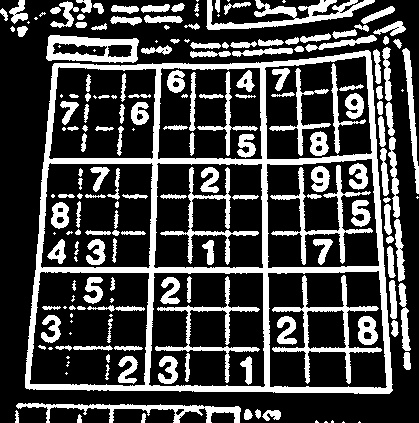
\includegraphics[width=\linewidth] {../../test/threshold/1.jpg}
        \caption{Input image}\label{fig:sht_example:a}
    \end{subfigure}\hfill
    \begin{subfigure}{0.3\textwidth}
        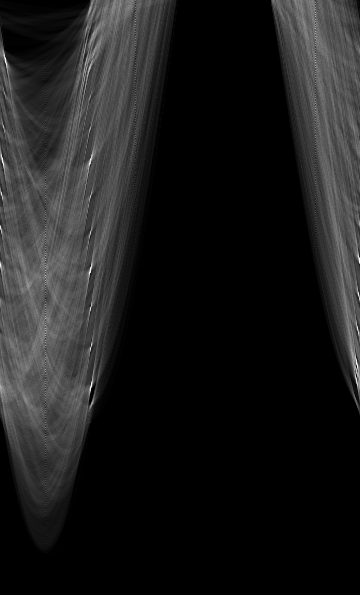
\includegraphics[width=\linewidth] {../../packages/js-benchmarks/img/seq.png}
        \caption{Accumulator}\label{fig:sht_example:b}
    \end{subfigure}\hfill
    \begin{subfigure}{0.3\textwidth}
        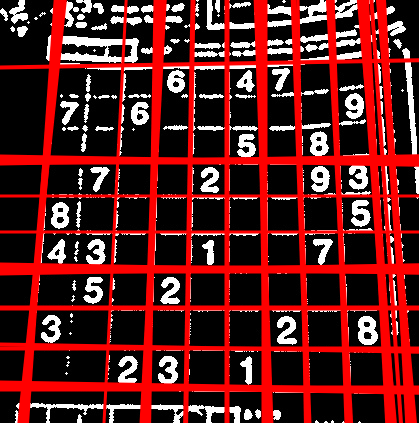
\includegraphics[width=\linewidth] {img/sht_result.png}
        \caption{Detected lines}\label{fig:sht_example:c}
    \end{subfigure}
    \caption{Input image, accumulator and visualized result of sequential SHT algorithm in non-LUT variant ($S_\theta = 1, S_\rho=1$).}\label{fig:sht_example}
\end{figure}




TODO: Implemented SHT, Non-LUT and LUT variants

TODO: Env x Methods matrix


TODO: library interface and building method

TODO: Comparing benchmarks across environments and methods, js sequential and C++ as reference point

TODO: JIT and cold/warm start, real-world vs synthetic

- TODO: CoV

- TODO: possibility of function extraction

TODO: Testing environment

- TODO: Hybrid CPU architecture and bench details

